 \documentclass[12pt]{article}
\usepackage[ruled,vlined]{algorithm2e}
\usepackage{amsmath}
\usepackage{amsfonts}
\usepackage{comment}
\usepackage{enumerate}
\usepackage[top=1in, bottom=1in, left=0.8in, right=1in]{geometry}
\usepackage{listings}
\usepackage{multicol}

\usepackage{tikz}
\usetikzlibrary{positioning}

\usepackage{wrapfig}

\lstset{language=Java, basicstyle={\small\ttfamily}, columns=flexible, belowskip=0mm}
\setlength{\columnsep}{0.1pc}

\begin{document}
\noindent
CS 344 \hfill \textbf{Problem Set 3} \newline 
{Fall 2020} \hfill \textbf{Due:} Nov 23, 2020, 11:59 p.m.

\noindent
\rule{\linewidth}{0.4pt}
\vspace{.4cm}

\textbf{Name}: ({\color{blue}Yuting Chen})~~~~~\textbf{NetID}: ({\color{blue}yc1071})

\vspace{.5cm}

\textbf{Honor Code}: Students may discuss and work on homework problems in groups, which is encouraged. However, each student must write down their solutions independently to show they understand the solution well enough to reconstruct it by themselves.  Students should clearly mention the names of the other students who offered discussions. We check all submissions for plagiarism. We take the honor code seriously and expect students to do the same.


\vspace{.5cm}

\textbf{Instruction for Submission}: This homework has a total of 100 points + 20 bonus points, it will be rescaled to 10 points + 2 bonus points as the eventual score. We have provided the homework3.tex file for you, please write your answer to each question in this latex file directly after the corresponding question, and submit the complied PDF file only. You should name your PDF file as ``{\color{blue}{Firstname-Lastname-NetID.pdf'}}'.

\vspace{.5cm}

\textbf{Late Policy}: The homework is due on 11/23 (Monday) at 11:59pm. We will release the solutions of the homework on Canvas on 11/27 (Friday) 11:59pm. If your homework is submitted to Canvas before 11/23 11:59pm, there will no late penalty. If you submit to Canvas after 11/23 11:59pm and before 11/27 11:59pm (i.e., before we release the solution), your score will be penalized by $0.9^k$, where $k$ is the number of days of late submission. For example, if you submitted on 11/26, and your original score is 80, then your final score will be $80*0.9^3=58.32$ for $26-23=3$ days of late submission. If you submit to Canvas after 11/27 11:59pm (i.e., after we release the solution), then you will earn no score for the homework.

\vspace{.5cm}

\noindent
\textbf{Drawing graphs:} You might try \texttt{http://madebyevan.com/fsm/} which allows you to draw graphs with your mouse and convert it into \LaTeX  \,code:

\begin{center}
%%%%%%% GENERATED AUTOMATICALLY BY madebyevan.com/fsm/
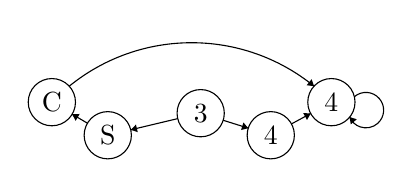
\begin{tikzpicture}[scale=0.1]
\tikzstyle{every node}+=[inner sep=0pt]
\draw [black] (26.7,-13.3) circle (3);
\draw (26.7,-13.3) node {C};
\draw [black] (45.6,-14.7) circle (3);
\draw (45.6,-14.7) node {$3$};
\draw [black] (33.8,-17.5) circle (3);
\draw (33.8,-17.5) node {S};
\draw [black] (54.5,-17.5) circle (3);
\draw (54.5,-17.5) node {$4$};
\draw [black] (62.2,-13.3) circle (3);
\draw (62.2,-13.3) node {$4$};
\draw [black] (42.68,-15.39) -- (36.72,-16.81);
\fill [black] (36.72,-16.81) -- (37.61,-17.11) -- (37.38,-16.14);
\draw [black] (31.22,-15.97) -- (29.28,-14.83);
\fill [black] (29.28,-14.83) -- (29.72,-15.67) -- (30.23,-14.8);
\draw [black] (48.46,-15.6) -- (51.64,-16.6);
\fill [black] (51.64,-16.6) -- (51.03,-15.88) -- (50.73,-16.84);
\draw [black] (57.13,-16.06) -- (59.57,-14.74);
\fill [black] (59.57,-14.74) -- (58.62,-14.68) -- (59.1,-15.56);
\draw [black] (28.907,-11.271) arc (129.11449:50.88551:24.638);
\fill [black] (59.99,-11.27) -- (59.69,-10.38) -- (59.06,-11.15);
\draw [black] (65.108,-12.614) arc (131.00538:-156.99462:2.25);
\fill [black] (64.51,-15.19) -- (64.66,-16.12) -- (65.42,-15.47);
\end{tikzpicture}
\end{center}

You can also draw by hand and insert a picture.

\vspace{.5cm}

\textbf{Make best use of picture in Latex}: If you think some part of your answer is too difficult to type using Latex, you may write that part on paper and scan it as a picture, and then insert that part into Latex as a picture, and finally Latex will compile the picture into the final PDF output. This will make things easier. For instructions of how to insert pictures in Latex, you may refer to the Latex file of our homework 1, which includes several examples of inserting pictures in Latex.


\hrulefill

Discussion Group (People with whom you discussed ideas used in your answers if any): Xudong Jiang    \\[1ex]


I acknowledge and accept the Honor Code. Please type your initials below:

\textbf{Signed}: ({\color{blue}YC})



\rule{\linewidth}{0.4pt}


\begin{enumerate}
  % Problem 1
  \item \textbf{Warmup with DFS/BFS.} (20 points)

(1) Give one example of a directed graph on four vertices, $A$, $B$, $C$, and $D$, such that both depth-first search and breadth-first search discover the vertices in the same order when started at A.  
\\{\color{blue}Answer: When DFS started at A, recover vertices in order ABCD. When BFS started at A, also recover vertices in order ABCD.
   \begin{figure}[h]
  	\centering
  	\includegraphics*[scale=0.1]{HW3-1.jpg}
	\caption{Question 1(a).}
	\label{fig:example}
  \end{figure}}

(2) Give one example of a directed graph where DFS and BFS discover the vertices in a different order when started at $A$.
{ \begin{figure}[h]
  	\centering
  	\includegraphics*[scale=0.1]{HW3-2.jpg}
	\caption{Question 1(b).}
	\label{fig:example}
  \end{figure}}
  \\{\color{blue}Answer: DFS started at A discovers vertices in order ABCD. BFS started at A does it in order ABCD.
  }

``Discover'' means the time that the algorithm first reaches the vertex, referred to as \verb|start_time| during lecture. Assume that both DFS and BFS iterate over outgoing neighbors in alphabetical order.

  \textbf{[We are expecting a drawing of your graphs and an ordered list of vertices discovered by DFS and BFS.]}

  % Problem 2
  \item \textbf{Warmup with Dijkstra.} (20 points)

  Let $G = (V,E)$ be a weighted directed graph.  For the rest of this problem, assume that $s, t \in V$ and that \textbf{there exists a directed path from $s$ to $t$}.

For the rest of this problem, refer to the implementation of Dijkstra's algorithm given by the pseudocode below.

\newpage

\begin{verbatim}
dijkstra_st_path(G, s, t):
  for all v in V, set d[v] = Infinity
  for all v in V, set p[v] = None 
  
  // we will use p to reconstruct the shortest s-t path at the end
  d[s] = 0
  F = V
  D = []
  while F isn't empty:
    x = vertex v in F such that d[v] is minimized
    for y in x.outgoing_neighbors:
      d[y] = min( d[y], d[x] + weight(x,y) )
      if d[y] was changed in the previous line, set p[y] = x
    F.remove(x)
    D.add(x)
        
  // use p to reconstruct the shortest s-t path
  path = [t]
  current = t
  while current != s:
    current = p[current]
    add current to the front of the path
  return path, d[t]
\end{verbatim}

The variable \verb|p| maintains the ``\textbf{p}arents'' of the vertices in the shortest s-t path, so it can be reconstructed at the end.

Step through \texttt{dijkstra\_st\_path}$(G,s,t)$ on the graph $G$ shown below. Complete the table below to show what the arrays \texttt{d} and \texttt{p} are at each step of the algorithm, and indicate what path is returned and what its cost is.

\begin{center}
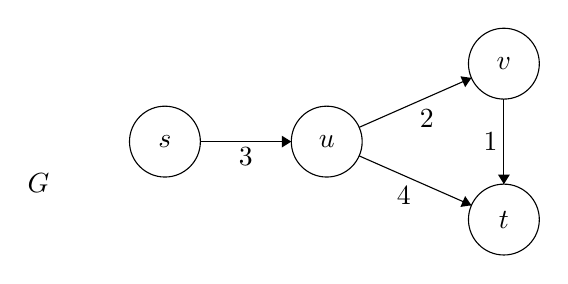
\begin{tikzpicture}[scale=0.15]
\tikzstyle{every node}+=[inner sep=0pt]
\draw [black] (20.7,-26.5) circle (3);
\draw (20.7,-26.5) node {$s$};
\draw [black] (34.4,-26.5) circle (3);
\draw (34.4,-26.5) node {$u$};
\draw [black] (49.4,-19.9) circle (3);
\draw (49.4,-19.9) node {$v$};
\draw [black] (49.4,-33.1) circle (3);
\draw (49.4,-33.1) node {$t$};
\draw [black] (23.7,-26.5) -- (31.4,-26.5);
\fill [black] (31.4,-26.5) -- (30.6,-26) -- (30.6,-27);
\draw (27.55,-27) node [below] {$3$};
\draw [black] (37.15,-25.29) -- (46.65,-21.11);
\fill [black] (46.65,-21.11) -- (45.72,-20.97) -- (46.12,-21.89);
\draw (42.88,-23.71) node [below] {$2$};
\draw [black] (49.4,-22.9) -- (49.4,-30.1);
\fill [black] (49.4,-30.1) -- (49.9,-29.3) -- (48.9,-29.3);
\draw (48.9,-26.5) node [left] {$1$};
\draw [black] (37.15,-27.71) -- (46.65,-31.89);
\fill [black] (46.65,-31.89) -- (46.12,-31.11) -- (45.72,-32.03);
\draw (40.92,-30.31) node [below] {$4$};
\node at (10,-30) {$G$};
\end{tikzpicture}
\end{center}

    \textbf{[We are expecting the table below filled out, as well as the final shortest path and its cost.  No further justification is required.]}

%%%%%%%%%%%%%%%%%%%%%%%%%%%%%%%%%%%%%%%%%%%%%%%%%%%%%%%%%%%%%%%%%%%%%%%%%%%%%%%%
%%%%%%%% TABLE: Fill in your answers between the & symbols below  if    %%%%%%%%
%%%%%%%% you wish to take this LaTeX code for your solution.            %%%%%%%%
%%%%%%%%%%%%%%%%%%%%%%%%%%%%%%%%%%%%%%%%%%%%%%%%%%%%%%%%%%%%%%%%%%%%%%%%%%%%%%%%

\begin{center}
\def\arraystretch{1.5}
\newcommand{\td}{\texttt{d}}
\newcommand{\tp}{\texttt{p}}
\begin{tabular}{|p{6cm}||c|c|c|c||c|c|c|c|}
\hline
& \td[$s$] & \td[$u$] & \td[$v$] & \td[$t$] & \tp[$s$] & \tp[$u$] & \tp[$v$] & \tp[$t$] \\
\hline
When entering the first while loop for the first time, the state is:&
0 & $\infty$ & $\infty$ & $\infty$ & None & None & None & None \\
\hline
Immediately after the first element of $D$ is added, the state is: &
0 & $3$ & $\infty$ & $\infty$ & None & s & None & None \\
 \hline
Immediately after the second element of $D$ is added, the state is: &
\color{blue}0 &\color{blue}$3$ & \color{blue}$5$ & \color{blue}$7$ & \color{blue}None & \color{blue}s & \color{blue}u & \color{blue}u \\
 \hline
Immediately after the third element of $D$ is added, the state is: &
\color{blue}0 &\color{blue}$3$ &\color{blue}$5$ &\color{blue}$6$ & \color{blue}None & \color{blue}s & \color{blue}u &\color{blue}v \\
 \hline
Immediately after the fourth element of $D$ is added, the state is: &
\color{blue}0 &\color{blue}$3$ &\color{blue}$5$ &\color{blue}$6$ &\color{blue}None &\color{blue}s &\color{blue}u &\color{blue}v \\
 \hline
\end{tabular}
\end{center}


%%%%%%%% END TABLE %%%%%%%%
{\color{blue} The final shortest path returned is $s \to u \to v \to t$, the cost is $d[t] = 6$. 
}


  % Problem 3
  \item \textbf{Fun with Reductions.}
(15 points) Suppose the  economies of the world use a set of currencies $C_1,\ldots,C_n$; think of these as dollars, pounds, Bitcoin, etc. Your bank allows you to trade each currency $C_i$ for any other currency $C_j$, and finds some way to charge you for this service. Suppose that for each ordered pair of currencies $(C_i,C_j)$, the bank charges a flat fee of $f_{ij} > 0$ dollars to exchange $C_i$ for $C_j$ (regardless of the quantity of currency being exchanged).

      Describe an algorithm which, given a starting currency $C_s$, a target currency $C_t$, and a list of fees $f_{ij}$ for all $i,j \in \{1,\ldots,n\}$, computes the cheapest way (that is, incurring the least in fees) to exchange all of our currency in $C_s$ into currency $C_t$.  Also, justify the its runtime.

      \textbf{[We are expecting a description or pseudocode (either is OK) of your algorithm, as well as a brief justification of its runtime. You can use any algorithm we have learned in class.]}
      
    \\{\color{blue}Answer: According to the question we know that we have n currencies, and we must convert from one currency to another currency, A fixed fee will be charged every time you exchanged in your banks. So we basically need to take measures to minimize the cost. This is basically a problem with the shortest path algorithm. We can use Dijkstra Algorithm to solve. 
    \\
    \\let Q is a queue of all nodes in the graph. when the algorithm's progress end, Q would be empty.S is an empty set to indicate which nodes the algorithm has visited. when the algorithm's run end, S would contain all the nodes of the graph. Vertices denoted by v, nodes denoted by u.
    \\Pseudocode:
    \\Dijkstra(Graph, currency)
    \\ distant[currency]  := 0;                   
    \\for (each vertex v in Graph)    
    \\if (v ≠ currency)
    \\distant[v]  := infinity;           
    \\add v to Q;   
    \\endif;
    \\endfor;
    \\while (Q is not empty)             
    \\v := vertex in Q with min distant[v];  
    \\remove v from Q;
    \\   for (each neighbor u of v )     
    \\       alt := distant[v] + length(v, u);
    \\     if (alt < distant[u])           
    \\       distant[u]  := alt ;
    \\endif;
    \\endfor;
    \\return distant[];
    \\endwhile;
    
    \\The cost of a path between two vertices in G is the sum of the weights of the vertices on that path. We show that, for such graphs, the time complexity of Dijkstra's algorithm, implemented with a binary heap, the runtime is $O(|E|+|V|log|V|)$.


    }


  % Problem 5
  \item \textbf{Social engineering.} (15 points + 10 bonus points)

  Suppose we have a community of $n$ people.  We can create a directed graph from this community as follows: the vertices are people, and there is a directed edge from person $A$ to person $B$ if $A$ would forward a rumor to $B$. Assume that if there is an edge from $A$ to $B$, then $A$ will always forward any rumor they hear to $B$. Notice that this relationship isn't symmetric: $A$ might gossip to $B$ but not
vice versa. Suppose there are $m$ directed edges total, so $G = (V,E)$ is a graph with $n$ vertices and $m$ edges.

  Define a person $P$ to be \em influential \em if for all other people $A$ in the community, there is a directed path from $P$ to $A$ in $G$.  Thus, if you tell a rumor to an influential person $P$, eventually the rumor will reach everybody. You have a rumor that you'd like to spread, but you don't have time to tell more than one person, so you'd like to find an influential person to tell the rumor to.
  
  In the following questions, assume that $G$ is the directed graph representing the community, and that you have access to $G$ as an array of adjacency lists: for each vertex $v$, in $O(1)$ time you can get a pointer to the head of the linked lists $v$\texttt{.outgoing\_neighbors} and $v$\texttt{.incoming\_neighbors}.  Notice that $G$ is not necessarily acyclic. In your answers, you may appeal to any statements we have seen in class, in the notes, or in CLRS.
  
  \begin{enumerate}
    \item (15 points) Show that all influential people in $G$ are in the same strongly connected component, and that everyone in this strongly connected component is influential.
      
    \textbf{[Hint: You need to refer the definition of strongly connected component, and you can prove using either induction or contradiction.]}
    \\{\color{blue}Answer:\color{blue} If v and v' are influential,  there is a path from v to V' and from v' to v. Therefore, according to the definition, v and v' are in the same strongly connected component. As same, if v is influential and v' is in the same SCC as v, v' is influential. because there is a path from v' to v to u, for all u \in V. 
    
}
    \item (10 bonus points) Suppose that an influential person exists. Give an algorithm that, given $G$, finds an influential person.
    
    \textbf{[We are expecting a description or pseudocode of your algorithm and a short argument about the runtime. You can borrow any algorithm that we have learned in class.]}
    \\{\color{blue}Answer:
    \\Pseudocode:
    \\influentialPerson(G)
    \\L=v;
    \\ \textbf{while} (L is not empty)
    \\v = any vertex in L;
    \\VISTED = [];
    \\DFStruncated (VISITED, $L$, $v$);
    \\remove all the vertices in VISITED from L;
    \\ \textbf{return v};
    \\endwhile;
    \\DFStruncated(VISITED, L, s)
    \\ \textbf{if}($s == NULL$ || $s$ is not in L)
    \\ \textbf{return};
    \\endif;
    \\VISITED.add(s);
    \\ \textbf{for} ($v$ in s.neighbors)
    \\DFStruncated(VISITED, L, v);
    \\endfor;
    \\
    \\In all DFStruncated calls, each vertex is only added to one VISITED, because once it has been visited in a call of DFStruncated, it is added to VISITED  and subtracted from L; it will never be DFStruncated access. Since DFStruncated only traverses directed adges(u, v), if it add u to the VISITED, it means that each directed edge is traversed only once. Therefore, the runtime is O(m+n).

     }
  \end{enumerate}


  \item \textbf{Job Sequencing Problem.} (15 points)

In this problem we have $n$ jobs $j_1, j_2, ..., j_n$, each has an associated deadline $d_1, d_2, ..., d_n$ and profit $p_1, p_2, ..., p_n$. Profit will only be awarded or earned if the job is completed before the deadline. We assume that each job takes 1 unit of time to complete. The objective is to earn maximum profit when only one job can be scheduled or processed at any given time.

Describe or provide the pseudocode of an algorithm to find the sequence of jobs to do with the maximum total profit.

    \textbf{[Hint: You can select the jobs in a greedy way. You can use the following example to help your analysis.]}

\begin{table}[h]
\hspace{5cm}
\begin{tabular}
{|c|c|c|c|c|c|}\hline
Job & J1 & J2 & J3 & J4 & J5\\\hline
Deadline & 2 & 1 & 3 & 2 & 1\\\hline
Profit & 60 & 100 & 20 & 40 & 20\\\hline
\end{tabular}
\end{table}

The best job sequence would be $J2 \rightarrow J1 \rightarrow J3$.
\\{\color{blue}Answer:
\\For this question, If we look at job j2, it has a deadline 1. This means we have to complete job j2 in time slot 1 if we want to earn its profit.As same, if we look at job j1 it has a deadline 2. This means we have to complete job j1 on or before time slot 2 in order to earn its profit.
\\Pscudocode:
\\ \textbf{for} ($i = 1$; $i<=n$, $i++$) do
\\Set j = min(deadlineMax, Deadline(i));
\\ \textbf{while} $j >= 1$ do
\\ \textbf{if} (timeSlot[j] is EMPTY)
\\timeSlot[j] = Job(i);
\\ \textbf{break};
\\endif;
\\Set j = j - 1;
\\endwhile;
\\endfor;

}
\item \textbf{Alternative Minimum Spanning Trees (23.4 CLRS).} (15 points + 10 bonus points)
In this problem, we give pseudocode for two different algorithms. Each one takes a connected graph and a weight function as input and returns a set of edges T. For each algorithm, either show that T is a minimum spanning tree (give a brief justification of the algorithm) or show that T is not a minimum spanning tree (give a counter-example).

a. (15 points) \textbf{MAYBE-MST-A} ($G, w$)\\
1. sort the edges into non-increasing order of edge weights $w$\\
2. $T = E$\\
3. for each edge $e\in E$, taken in non-increasing order by weight\\
4.~~if $T - \{e\}$ is a connected graph\\
5.~~~~$T = T - \{e\}$\\
6. return $T$\\
\\{\color{blue}Answer: MAYBE-MST-A is a MST algorithm. As we know that we cannot remove an edge that must be part of a minimum spanning tree. so we cannot remove e that is a bridge. We only remove an edge e if T-{e} is a connected graph and e lies on a simple cycle of the graph. Since we remove edges in non-increasing order, the weight of every edge on the cycle must be less than or equal to e. so the output T is composed of a minimum number of edges of minimum weight, and is valid MST. This is a minimum spanning tree on G with edge e removed.

}

b. (10 bonus points) \textbf{MAYBE-MST-B} ($G, w$)\\
1. $T = null$\\
2. for each edge $e$, taken in arbitrary order\\
3.~~ if $T \cup \{e\}$ has no cycles\\
4.~~~~$T = T \cup \{e\}$\\
5. return $T$\\

\\{\color{blue} Answer: MAYBE-MST-B is not a MST algorithm. If the algorithm examines the edges in their order listed, the algorithm never adjusts edges or removes edges. Because of the arbitrary order. We could add any edge e to the MST. The heavy edge did not make a cycle when lighter edges would be more optimal. For example, let G be the graph on 3 vertices a, b, and c. The edges be (a,b)with weights 3. The edges be (b,c)with weights 2, The edges be (c,a)with weights 1. So it would take the two heaviest edges when the algorithm examines the edges in their order listed. T is not a minimum spanning tree.
}


\end{enumerate}

\end{document}